\section{Introduction}
\label{sec:introdction}
Data exploration has gained lots of attentions over the last few years. The
main challenge is to support users with no clear requirements. To solve it,
several authors have proposed systems to ``play'' with the
data~\cite{abouzied2012dataplay, sellam2013meet, liarou2014dbtouch,
dimitriadou2014explore}. Typically, these systems propose some graphical
interface through which users can create, visualize and modify selections of
tuples quickly. Thus, users are engaged in a tight trial-and-error loop,
through which they discover their datasets.\\
These approaches are designed to help discovery. And indeed, they assume little
about the user's preliminary knowledge of the data. Yet, they rely on a crucial
assumption: they suppose that if a user sees an interesting set of tuples
(e.g., through tables or visualizations), they will recognize it immediately,
and think ``aha, this is interesting''. This assumption may hold with small
datasets, but it breaks down in higher dimensions. The first bottleneck is the
time necessary to inspect each column on after the other. The second one  is
humans' perception of high dimension spaces:  we cannot reasonably expect a
user to grasp more than three, maybe four dimensions. 

To cope with this problem, we suggest that the exploration system should
\emph{describes} the tuples, in a language that users can understand. This
leads us to our problem statements:
\begin{framed}
    \everypar={{\setbox0=\lastbox}\everypar{}}
How can we describe a given set of tuples with natural language?
\end{framed}
In this paper, we introduce our algorithm, Ziggy. Ziggy's approach is to detect
subspaces for which the selected tuples are ``special'', i.e., have an unusual
distribution compared to the rest of the database. Then, for each of these
subspaces, it generates a natural language description of their distribution,
using statistical tests and hand-crafted rules. Here is an example of
description:
\begin{quote}
    Take a look at columns X, Y and Z. On X, and Y, your selection has a very
    low value. On column Z, your selection has a fairly low value, with high
    concentration. The correlation between Y and Z is unusually strong.\\
    You can also take a look at columns T. On this column, the
    values ``xxx'', ``yyy'', and ``ttt'' are underrepresented, while the values
    ``aa'' and ``bb'' are overrepresented.
\end{quote}

Several authors have tackled similar problems in the
past~\cite{angiulli2009detecting, knorr1999finding, loekito2008mining,
webb2008detecting}. None of them use natural language.

Our paper is built as follows. First, we discuss how to detect database views
in which a given set of tuple is ``special''. We expose the problem in its
generality, and discuss its relation to other methods, such as feature
selection. Second, we instantiate our problem with a custom objective function,
designed to yield interpretable results. Our function aggregates several
well-known statistical tests, carried out in a systematic, purposely
brute-force way.  Finally, we discuss how to describe the views with natural
language, and how to check the robustness of our results.

\section{General Problem Formulation}
\label{sec:problem}

\begin{figure}
  \centering
  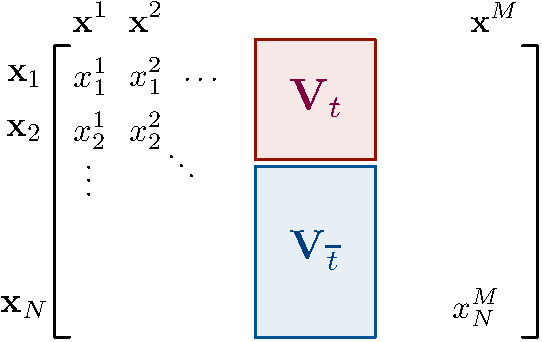
\includegraphics[width=0.6\columnwidth]{Figures/Notations}
  \caption{Notations.}
  \label{pic:notations}
\end{figure}
Let the matrix $\rb{D}$ with $M$ columns and $N$ rows represent our database.
We suppose that each tuple $\rb{x}_n = (x^1_n, \dots, x^M_n)^\top$ in the
database is an iid. sample from some unknown distribution
$p(\rb{x}_n)=p(\rb{x})$. We represent each column with a vector $\rb{x}^{m}=
(x^m_1, \dots, x^m_N)^\top$.  The user specifies a ``special'' selection of
tuples, described by the vector $\rb{t} = (t_1, \ldots, t_n)^\top$: $t_i=1$ if
the tuple is chosen, 0 otherwise. We refer to the tuples in the selection as
${\rb{D}}_t$, and the remaining tuples as ${\rb{D}}_{\overline{t}}$. We refer
to the underlying distributions as $p(\rb{x}|t)$ and $p(\rb{x}|\overline{t})$
respectively. We illustrate these notations with Figure~\ref{pic:notations}.

Our model is based on a user-specified \textbf{mass dissimilarity measure}
$\mf{D}(\rb{D}, \rb{D}')$, which measures the difference between two groups of
tuples. If the rows of $\rb{D}$ and $\rb{D}'$ are sampled from the same
distribution, then $\mf{D}$ is very close to 0. If
not, $\mf{D}$ grows with the dissimilarity of the distributions.
Figure~\ref{pic:sameMean} gives an example of the latter case.  Here are some
possible choices:
\begin{itemize}
    \item A simple option is to use the distance between centroids (possibly
        weighted by the observed covariance)
    \item A more general option is to estimate the Kullback-Leibler divergence:
        $\mf{D}(\rb{D}, \rb{D}') \equiv KL(\hat{p}(\rb{x});
        \hat{p}'(\rb{x}'))$, where $\hat{p}(\rb{x})$ and $\hat{p}'(\rb{x}')$
        are density estimators. This approach is more general, as it can cope
        with both continuous and categorical variables.
    \item In the next section, we introduce our own mass dissimilarity.
\end{itemize}
Knowing this function $\mf{D}$, we can already propose a first, naive,
formulation of our problem. \emph{We want to find groups of variables on which the
distribution of the chosen tuples is different from that of the rest of the
data}.
\begin{problem}
    Consider a distribution dissimilarity function $\mf{D}$ and two integers
    $K$ and $D$. Find the top $K$ distinct views $\rb{D}^i = [\rb{x}^1, \dots,
    \rb{x}^d]$ with at most $D$ dimensions which maximize: $ \mf{D}\big(
    \rb{D}^i_t ; \rb{D}^i_{\overline{t}} \big)$ (ignoring column permutations).
\end{problem}
\begin{figure}
  \centering
  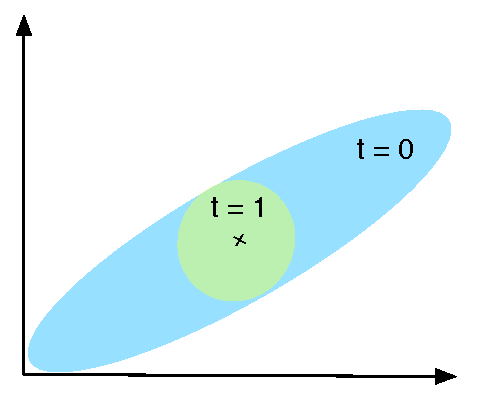
\includegraphics[width=0.8\columnwidth]{Figures/SameMean}
  \caption{Example of interesting view.}
  \label{pic:sameMean}
\end{figure}
This approach is simple, but it can lead to lots of redundancy: a small number
of good columns may dominate the results and appear in all $K$ views. In a data
exploration scenario, users may value \emph{diversity}, even if the views are
sub-optimal. To enforce this requirement, we introduce a penalty factor in our
objective function.

To measure redundancy, we need a \textbf{dependency measure} $\mf{S}$, which
measures the statistical dependency between the underlying distributions of two
sets of tuples $\rb{D}$ and $\rb{D}'$.  Here are some possible choices:
\begin{itemize}
    \item We can use a simple linear coefficient, or a its multivariate
        generalization, the RV-coefficient.
    \item Alternatively, we can estimate the mutual information of the
        underlying variables:
        $\mf{S}(\rb{D}', \rb{D}') \equiv \hat{I}(\rb{x}, \rb{x'})$.
\end{itemize}
We can now introduce a new version of our problem. We seek views
which maximize the distance statistic, while minimizing inter-view dependency.
We define this problem in a recursive way:
\begin{problem}
    Suppose that we have already detected $i$ views. We obtain $\rb{D}^{1..i} =
    [\rb{D}^1, \ldots, \rb{D}^i]$ by concatenating these views.  Given a
    positive real $\lambda$, find the view $\rb{D}^{i+1}$ with at most $D$
    columns which maximizes:
        \begin{equation}
            \label{prob1}
            \mf{D}\big( \rb{D}^{i+1}_t  ; \rb{D}^{i+1}_{\overline{t}} \big) - 
            \lambda \cdot \mf{S} ( \rb{D}^{i+1} ; \rb{D}^{1..i})
        \end{equation}
\end{problem}
Observe that the parameter $\lambda$ controls the trade-off between mass distance
and view diversity. For some $L$, an equivalent way to express our problem is
the following:
\begin{equation}
    \label{prob2}
    \begin{aligned}
        & \text{Argmax}_{\rb{D}^{i+1}} 
            & \mf{D}\big( \rb{D}^{i+1}_t  ; \rb{D}^{i+1}_{\overline{t}} \big)\\
        & \text{s.t.} 
        &\mf{S} ( \rb{D}^{i+1} ; \rb{D}^{1..i}) & < L\\ 
    \end{aligned}
\end{equation}
Equation~\ref{prob1} in the Lagrangian of Equation~\ref{prob2}, up to an
additive constant.

At this point, we notice that our problem is very to close to \emph{feature
selection}. Feature selection seeks columns of $\rb{D}$ from which we can
predict $\rb{t}$. Ultimately, the goal is to estimate $p(t|\rb{x})$. Our
problem is symmetric: we seek columns of $\rb{D}$ which \emph{are predicted} by
$\rb{t}$.  Hence, we focus on $p(\rb{x}|t)$. According to Bayes' theorem, these
two problems are equivalent. And indeed, some feature selection methods, such
as LDA, are also based on $p(\rb{x}|t)$.

The differences do not stop here. Recall that Ziggy focuses on
\emph{interpretation}, while feature selection algorithms focus on
\emph{prediction}. Therefore, Ziggy returns a few, non-redundant views, while
classic algorithms focus on single, potentially complex views. Also, most
feature selection algorithms optimize \emph{class separability}. In this paper,
we are interested in \emph{any} kind of dissimilarity. For instance, most
feature selection algorithms would reject the view presented
in Figure~\ref{pic:sameMean}. For Ziggy, this view is perfectly acceptable. 

Finally, we may wonder what is the difference between Ziggy and Claude. After
all, they are quite similar. I discuss this point in the Appendix.


\section{Instantiation: Meet Ziggy}
\label{sec:instantiation}

\subsection{Explainable Mass Dissimilarity}
\label{sec:explain}

We now discuss how to instantiate the function~$\mf{D}$. In principle, we could
borrow a very general divergence measure from the statistics literature, such
as the KL-divergence.  Such instantiation, coupled with visualization
technology, would be perfectly suited to a expert user. Instead, we chose to
focus on non-experts. We introduce the \textbf{Zig-dissimilarity} (Ziggy's
Dissimilarity), an \emph{explainable} mass dissimilarity
measure.

To obtain the Zig-dissimilarity between two sets of tuples, we operate as
follows. First, we compute several univariate dissimilarity indicators $z^1,
\ldots, z^Z$.  Each of them highlights a specific difference between $\rb{D}_t$
and $\rb{D}_{\overline{t}}$, based on one-dimension statistics. For instance,
they describe the difference between means, or the ratio of the variances, for
each variable $\rb{x}^m$ separately.  We call them \textbf{zig-components}.  In
a second step, we compute bivariate zig-components. These describe possible
differences with regards to dependency: for instance, the regression line
between two variables may be steeper for our special tuples. Finally, we
concatenate all these scores in a vector $\rb{z}=(z^1_1, \ldots, z^Z_M)$, and
aggregate them using the norm $\norm{\rb{z}}_P=\left(\sum_{z \in \rb{z}} w_z
\cdot |z|^P \right)^{1/P}$, with optional weights $w_z$.

\begin{table*}[t!]
    \centering
    \begin{tabular}{|c|c|c|c|l|}
      \hline
      Property & Type 1 & Type 2 & Zig-component & Comments\\
      \hline
      Difference of means        & Contin.  & - &
        $\frac{\mu_T - \mu_{\overline{T}}}{ \sigma_{\overline{T}}}$ (Glass'
        $\Delta$) &  \\
    Difference of variances    & Contin.  & - &
        $ \frac{\sigma_T - \sigma_{\overline{T}}}{ \sigma_{\overline{T}}}$ & \\
    Difference of Frequencies & Discrete & - & 
        $\sqrt{\frac{\chi^2}{N(k - 1)}}$ (Cram\'er's V) & \\
      \hline
      Dependence  & Contin. & Contin & $ r_T - r_{\overline{T}} $ & $r$ is the
      correlation coefficient\\
      Dependence  & Discrete & Both & $ V_T - V_{\overline{T}} $ & $V$ is
      Cram\'er' V\\
      \hline
    \end{tabular}
\caption{Our choice of Zig-components for different data types. Note that in
the bivariate case we actually compute statistics of statistics.}
    \label{tab:dissim}
\end{table*}

We report the z-component we used in our study in Table~\ref{tab:dissim}.  Each
component describes an interpretable property of the data.  Most of them come
from the classic statistics literature, where they are referred to as
\emph{effect sizes}. Their value is 0 if there is not difference between the
full database and the tuple of interest. Their absolute value varies with the
magnitude of the effect.

Observe that we compute univariate, then bivariate statistics. In principle, we
could test spaces with more dimensions. We chose not to do so, for two
practical reasons. First, we suppose that relationships in three dimensions or
more are harder to convey and understand in natural language.  Second, the
number of relationships to be tested grows exponentially with the
dimensionality of the test (up to tests of dimension $M/2$). This harms Ziggy's
runtime, and it leads to much longer explanations.


\subsection{Dependency Measure}
\label{sec:dependency}

We now discuss how to instantiate the dependency measure~$\mf{S}$. We chose
following:
\begin{gather}
    \mf{S}(\rb{D}, \rb{D'}) = \max_{d \neq d'} \mf{s}(d, d'), \text{where:}\\
         \mf{s}(d, d')= \begin{cases}
             r(d, d') \text{(correlation) if $d$ and $d'$ are continuous}\\
             V(d, d') \text{(Cram\'er's V) otherwise}
         \end{cases}
\end{gather}
We chose this measure for two reasons. First, it is easily interpretable, as
relies on well-known statistics. Second, it is computationally efficient.
We get the correlations ``for free'', because we need to compute them
anyway for the Zig-dissimilarities. Besides, the \emph{max} function lets us
explore the search space rapidly, as we will show in the following sections.


\section{Model Validation}
\label{sec:validation}

We now focus on the following problem: how \emph{significant} are the
dissimilarities associated to our views? Let us consider the general
case. We want to test a view $\rb{D}$, with mass dissimilarity $d = \mf{D}(
\rb{D}_t  ; \rb{D}_{\overline{t}})$. A high value may indicate that  $\rb{D}_t$
and $\rb{D}_{\overline{t}}$ come from two different distributions. But it could
also be caused by chance. How confident are we of this result? Note that this
section deals with the \emph{aggregated} dissimilarity: in Ziggy's case, this
means that we want to test the Z-dissimilarity, not the individual
z-dissimilarities (in fact, we already know their significance).

The statistics literature provides us a completely generic way to solve this
problem: permutation testing. The idea is to shuffle the rows of $D$, without
modifying $\rb{t}$. Thus, the tuples are randomly affected to $\rb{D}_t$ and
$\rb{D}_{\overline{t}}$. We then measure the new distance $d=\mf{D}\big(
\rb{D}^{i+1}_t  ; \rb{D}^{i+1}_{\overline{t}} \big)$. We repeat the experiment
$B$ times, and obtain the results $d^1, \ldots, d^B$. We compare them to our
initial measurement $d$. If $p\%$ samples are greater than $d^0$, then our
p-value is approximately $p$.



\section{Experiments}
\label{sec:experiments}

\section{Conclusion}
\label{sec:conclusions}
